\chapter{METHODOLOGY}\label{sec3}
\vspace{-3em}

.\section{System Architecture}\label{subsec:arch}

Figure~\ref{fig:methodology} provides an overview of the four main components of SubchatTrees: 1.tree-based conversation structure, 2.local buffer management, 3.global vector memory, and 4.the RAG retrieval pipeline.








\clearpage
\thispagestyle{empty}
\begin{tikzpicture}[remember picture,overlay]
\node at (current page.center) {\rotatebox{90}{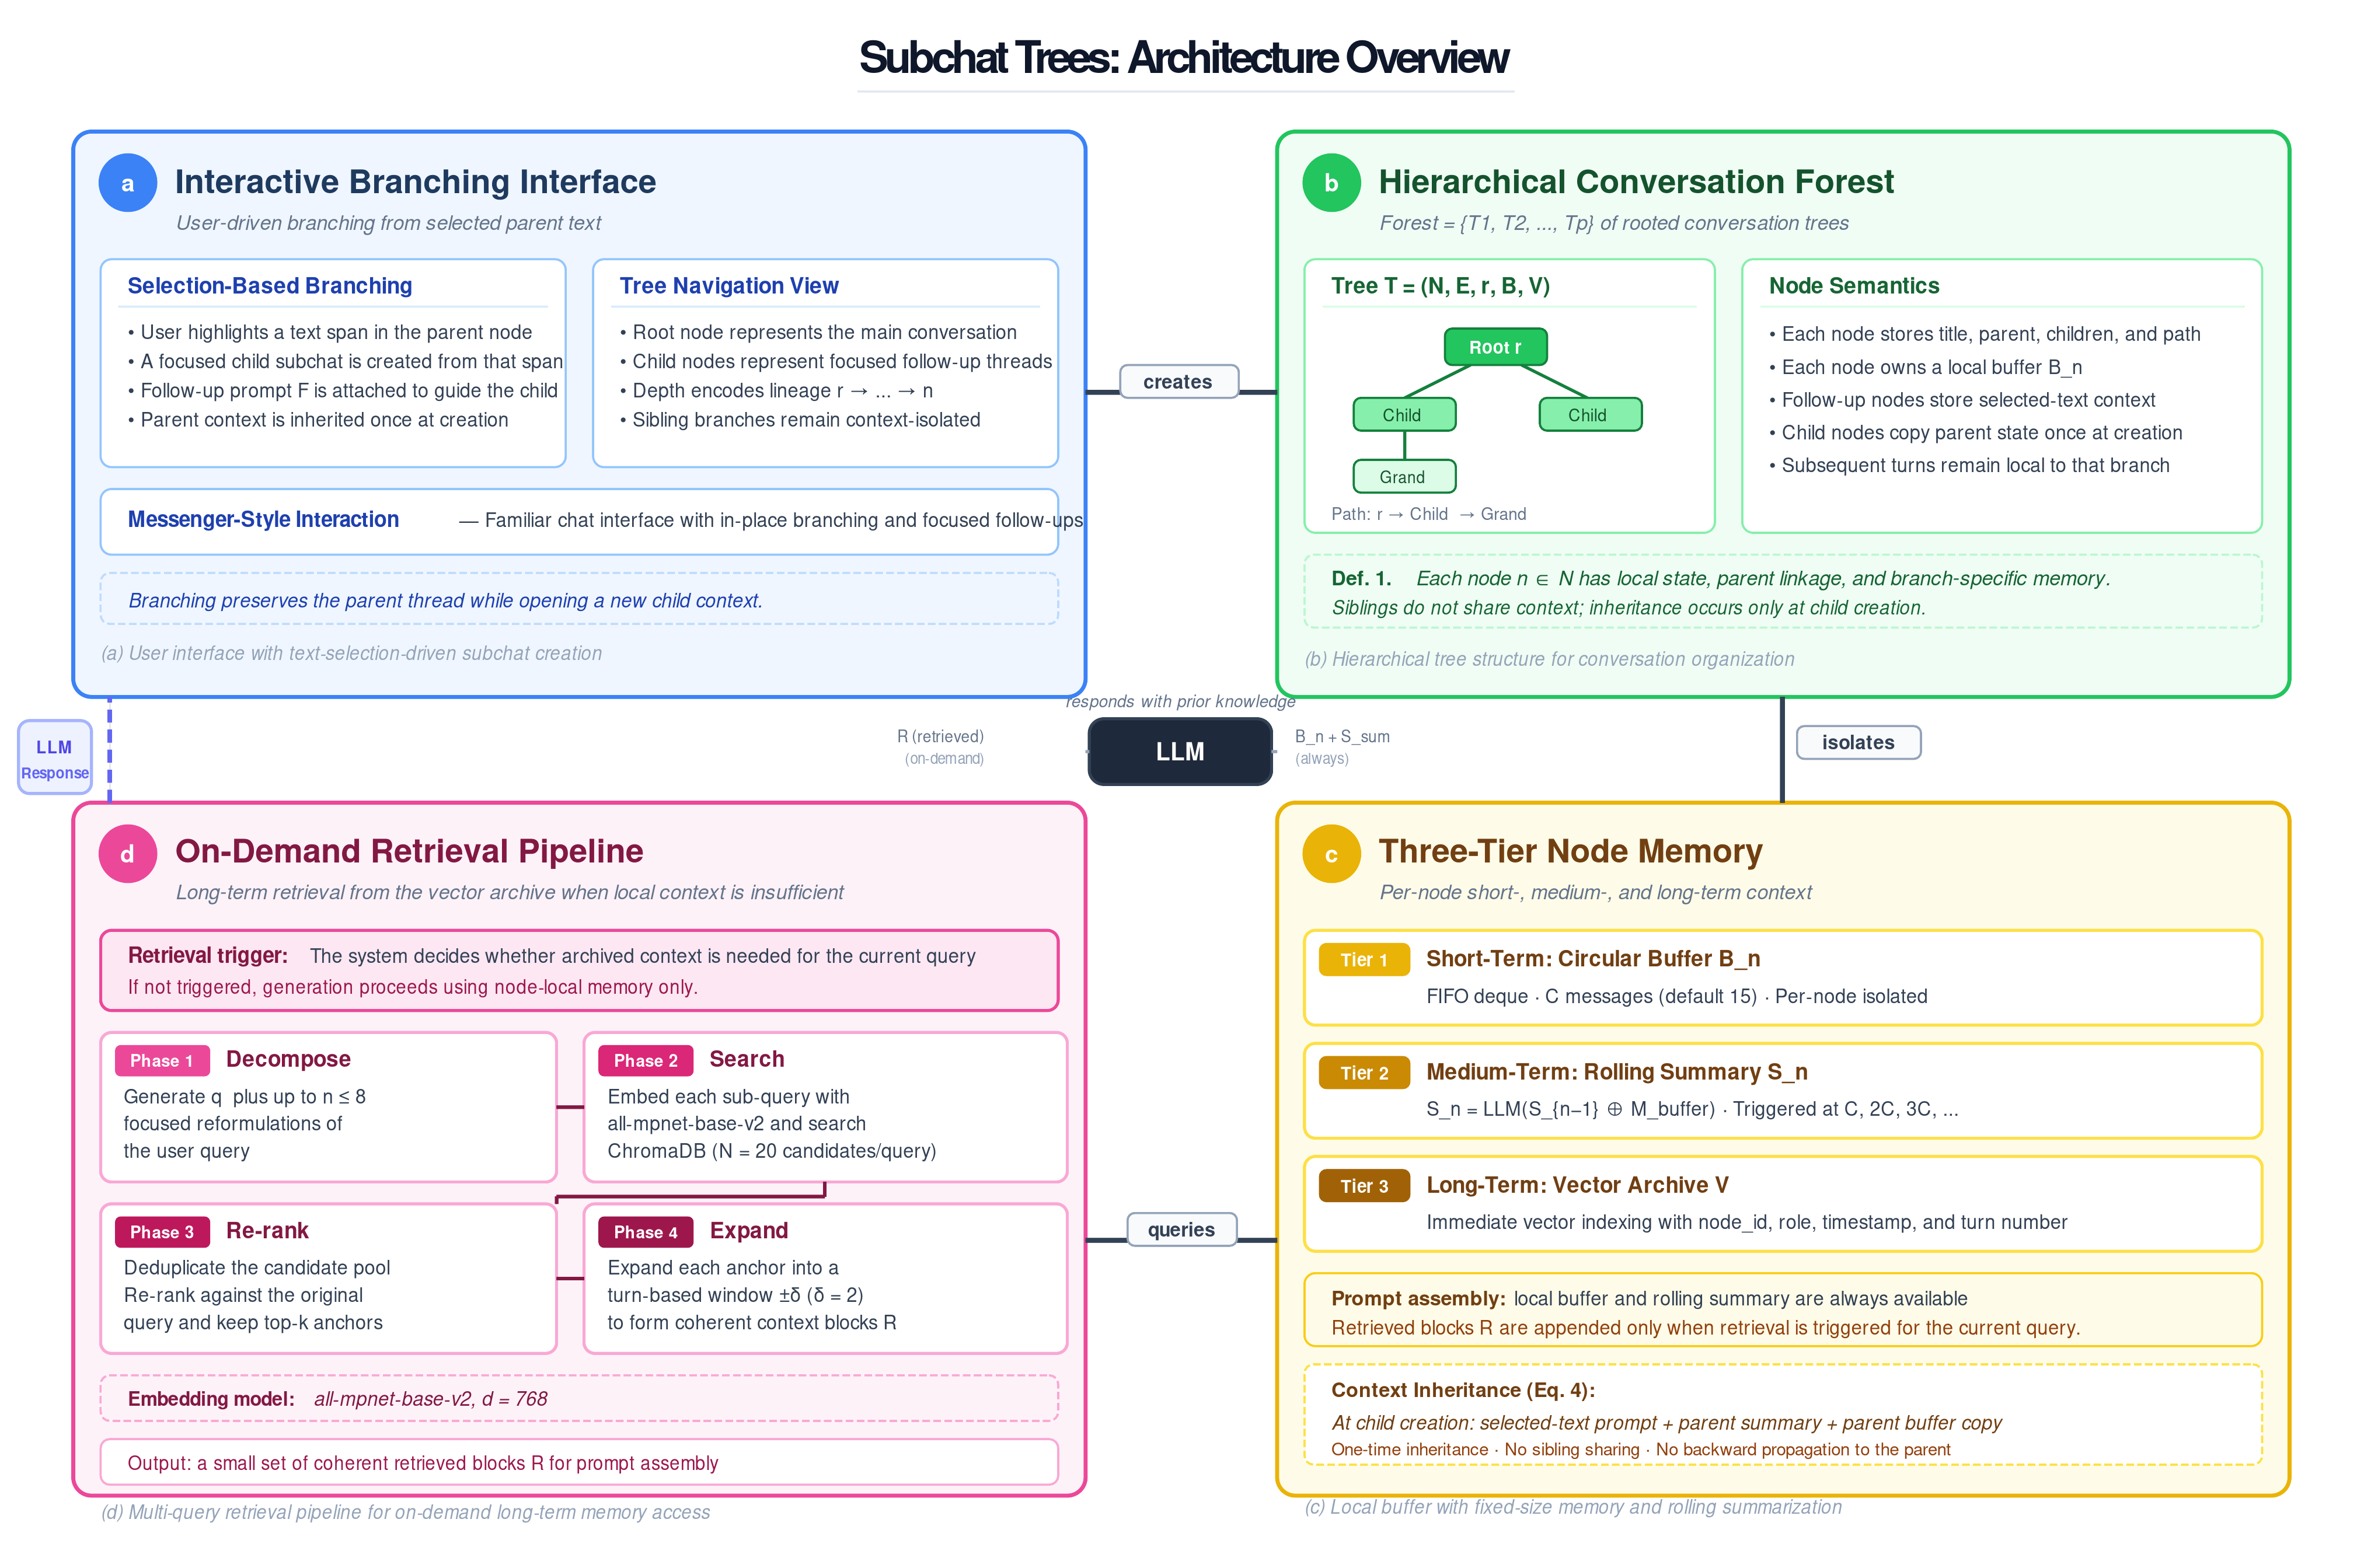
\includegraphics[width=0.90\paperheight,height=0.90\paperwidth,keepaspectratio]{diagrams/meth_latex_safe.png}}};
\end{tikzpicture}
\null
\clearpage
\captionof{figure}{Overview of the SubchatTrees methodology showing four components: (a) hierarchical tree structure for conversation organization, (b) local buffer with fixed-size memory management, (c) global vector store for long-term archival and (d) multi-query RAG pipeline for context retrieval.}
\label{fig:methodology}


\subsection{Hierarchical Conversation Tree Structure}\label{subsubsec:tree}

The system organizes conversations as hierarchical tree structures, where each node represents a distinct conversation thread with isolated context.





\begin{definition}[Conversation Tree]
A conversation tree $T$ is defined as a tuple of $(N, E, r, \mathcal{B}, \mathcal{V})$ here:
\begin{itemize}
    \item $N = \{n_1, n_2, \ldots, n_k\}$ set of conversation nodes,
    \item $E \subseteq N \times N$ set of directed parent$\to$child edges,
    \item $r \in N$  root node (main conversation),
    \item $\mathcal{B}: N \rightarrow B$ maps each node to its local buffer $B_i$,
    \item $\mathcal{V}: N \rightarrow \mathbb{R}^d$ maps each node's messages to $d$-dimensional embeddings space in a shared vector store.
\end{itemize}
\end{definition}

A \texttt{Forest} is a collection of independent trees $\mathcal{F} = \{T_1, T_2, \ldots, T_p\}$, allowing users to maintain isolate conversation threads (e.g., work projects, personal queries, research topics) without any cross-contamination. Figure~\ref{fig:forest} illustrates Hierarchical organization of Conversational Trees, composing the \texttt{conversation Forest}.





\clearpage
\thispagestyle{empty}
\begin{tikzpicture}[remember picture,overlay]
\node at (current page.center) {\rotatebox{90}{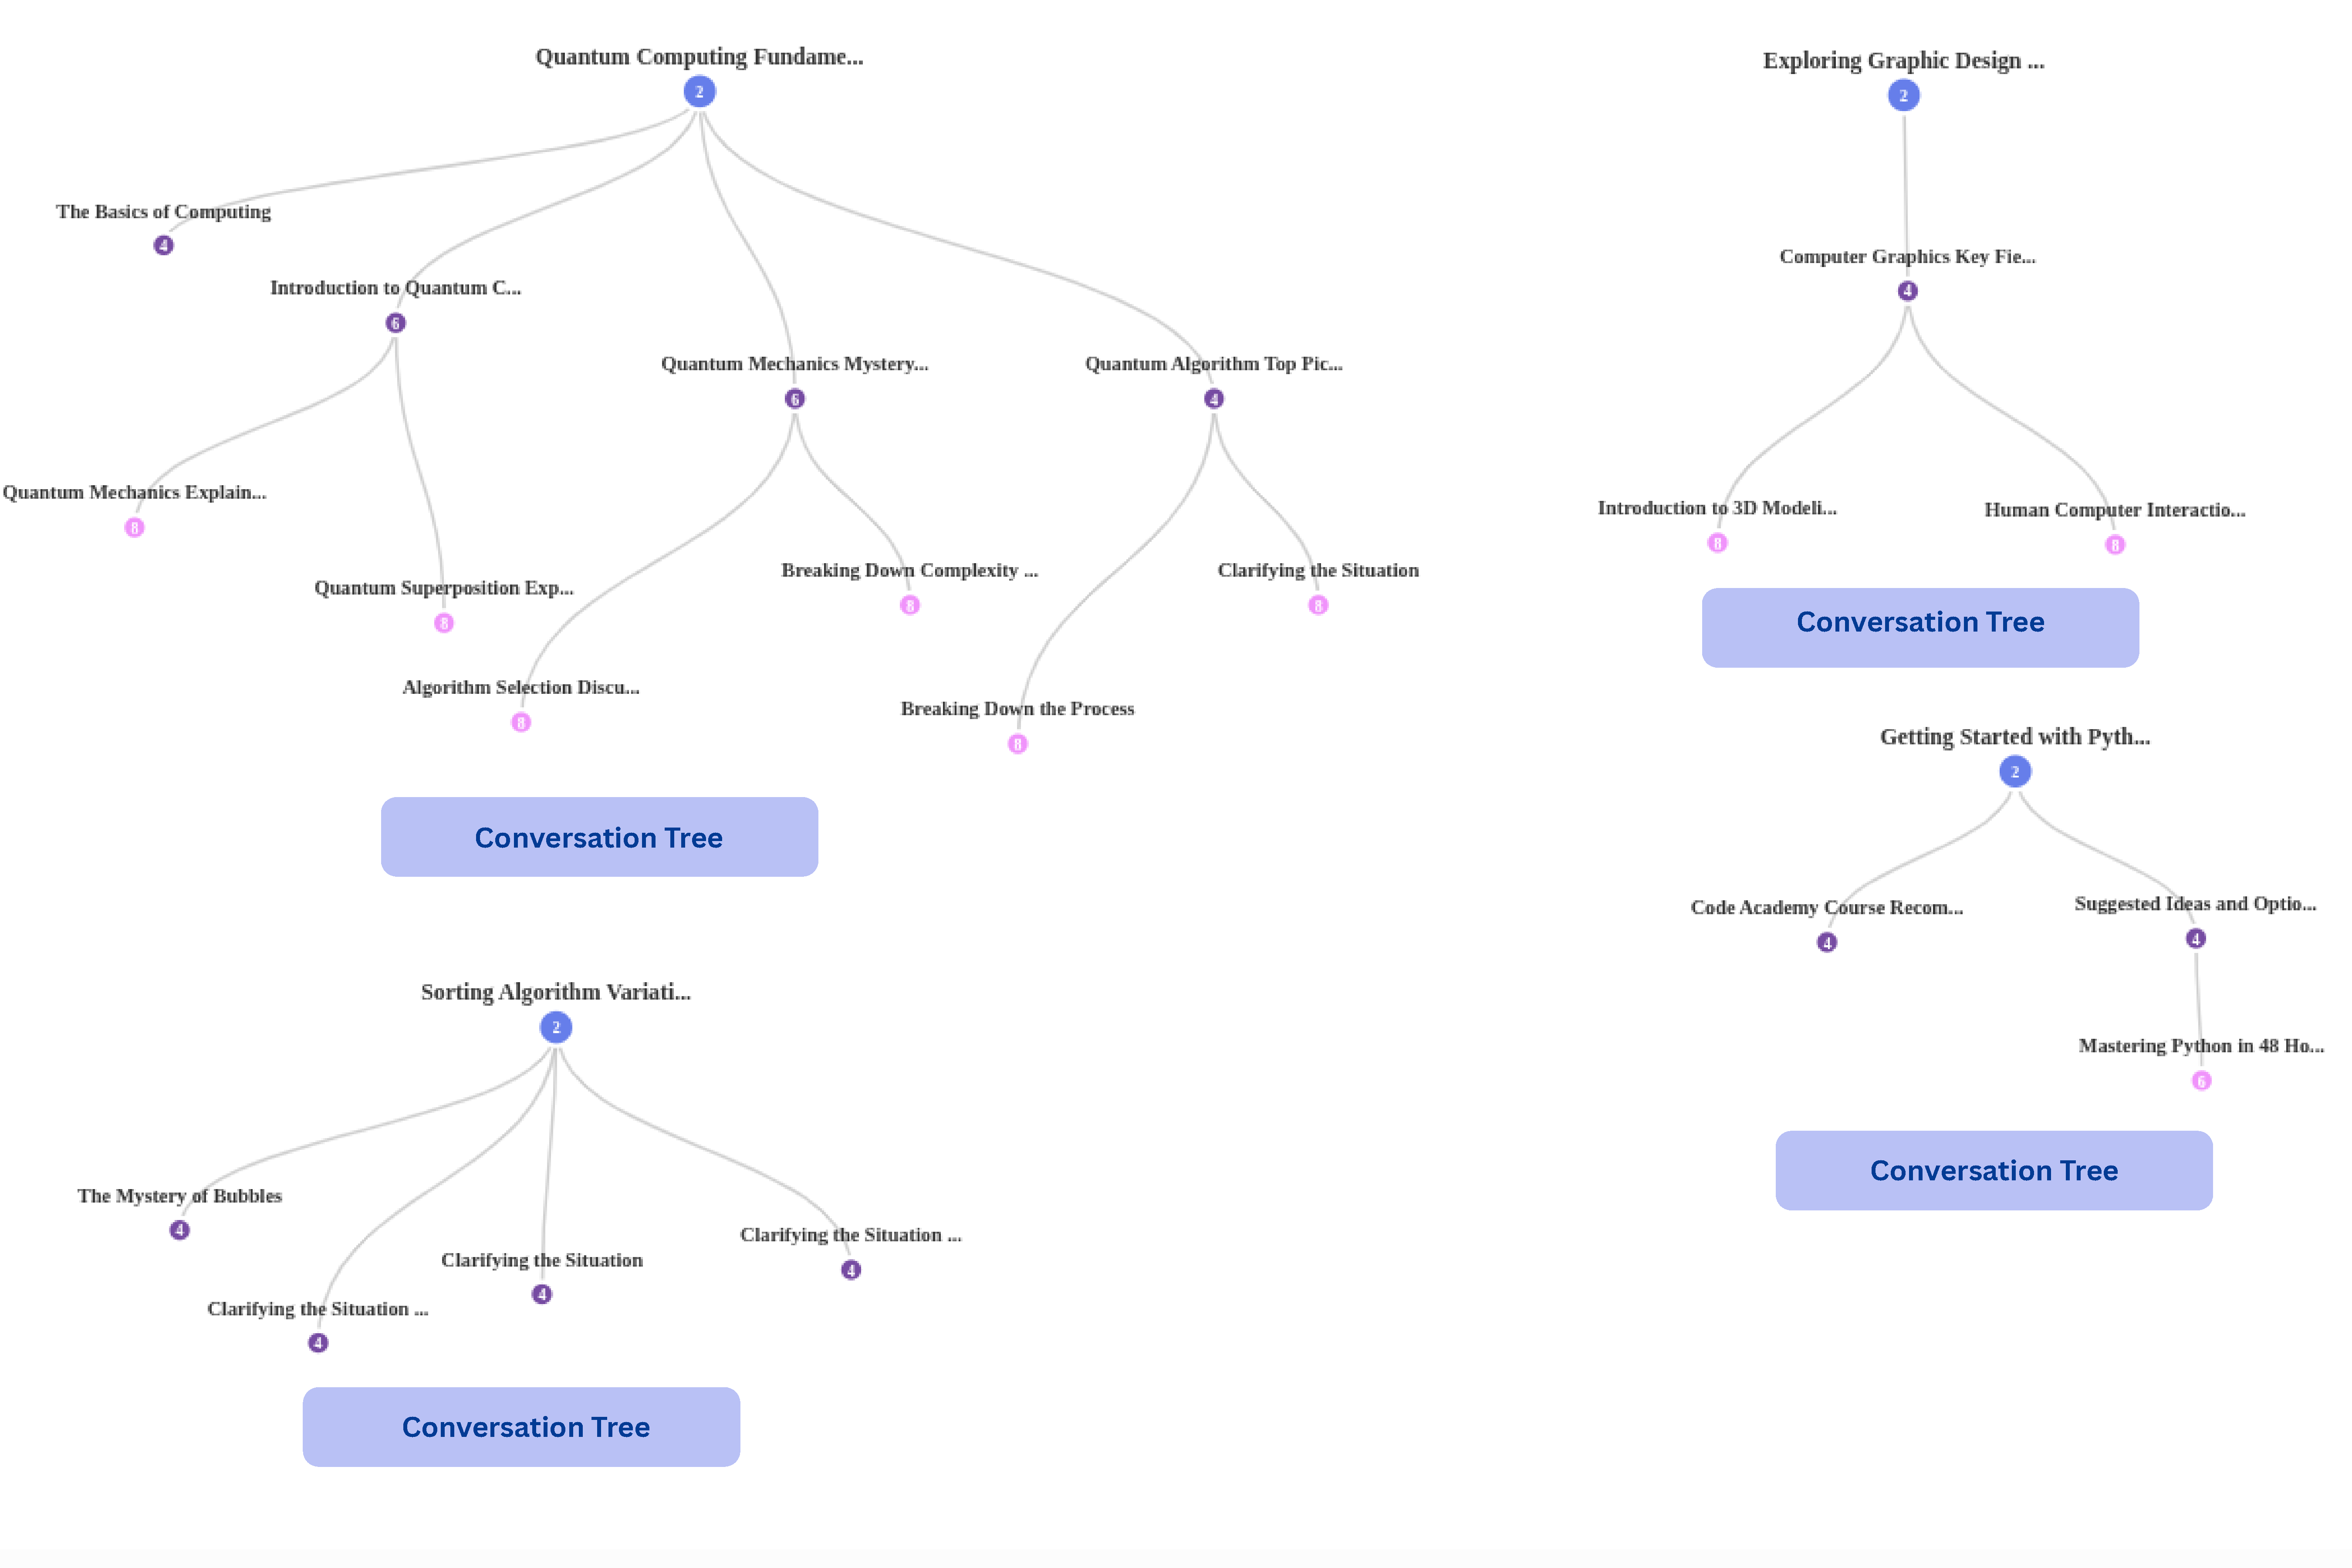
\includegraphics[width=0.90\paperheight,height=0.90\paperwidth,keepaspectratio]{diagrams/conversation tree.pdf}}};
\end{tikzpicture}
\null
\clearpage
\captionof{figure}{Tree view of a Conversation Forest showing multiple conversation branches. Each node represents a subchat with isolated context.}
\label{fig:forest}


Each \texttt{Tree} node $n_i$ maintains its own:
\begin{enumerate}
    \item \textbf{Local Buffer} $B_i$: a circular deque with configurable capacity $C$ (default $C{=}20$ messages).
    \item \textbf{Node Metadata:} unique identifier (\texttt{node\_id}), title, parent reference, children pointers.
    \item \textbf{Follow-up Context:} user intent behind branch creation and context type (\texttt{follow\_up}, \texttt{new\_topic}, or \texttt{general}).
\end{enumerate}

\subsection{Memory Management Strategy}\label{subsubsec:memory}

The memory architecture is divided into three complementary tiers, illustrated in Figure~\ref{fig:memory}.

\clearpage
\thispagestyle{empty}
\begin{tikzpicture}[remember picture,overlay]
\node at (current page.center) {\rotatebox{90}{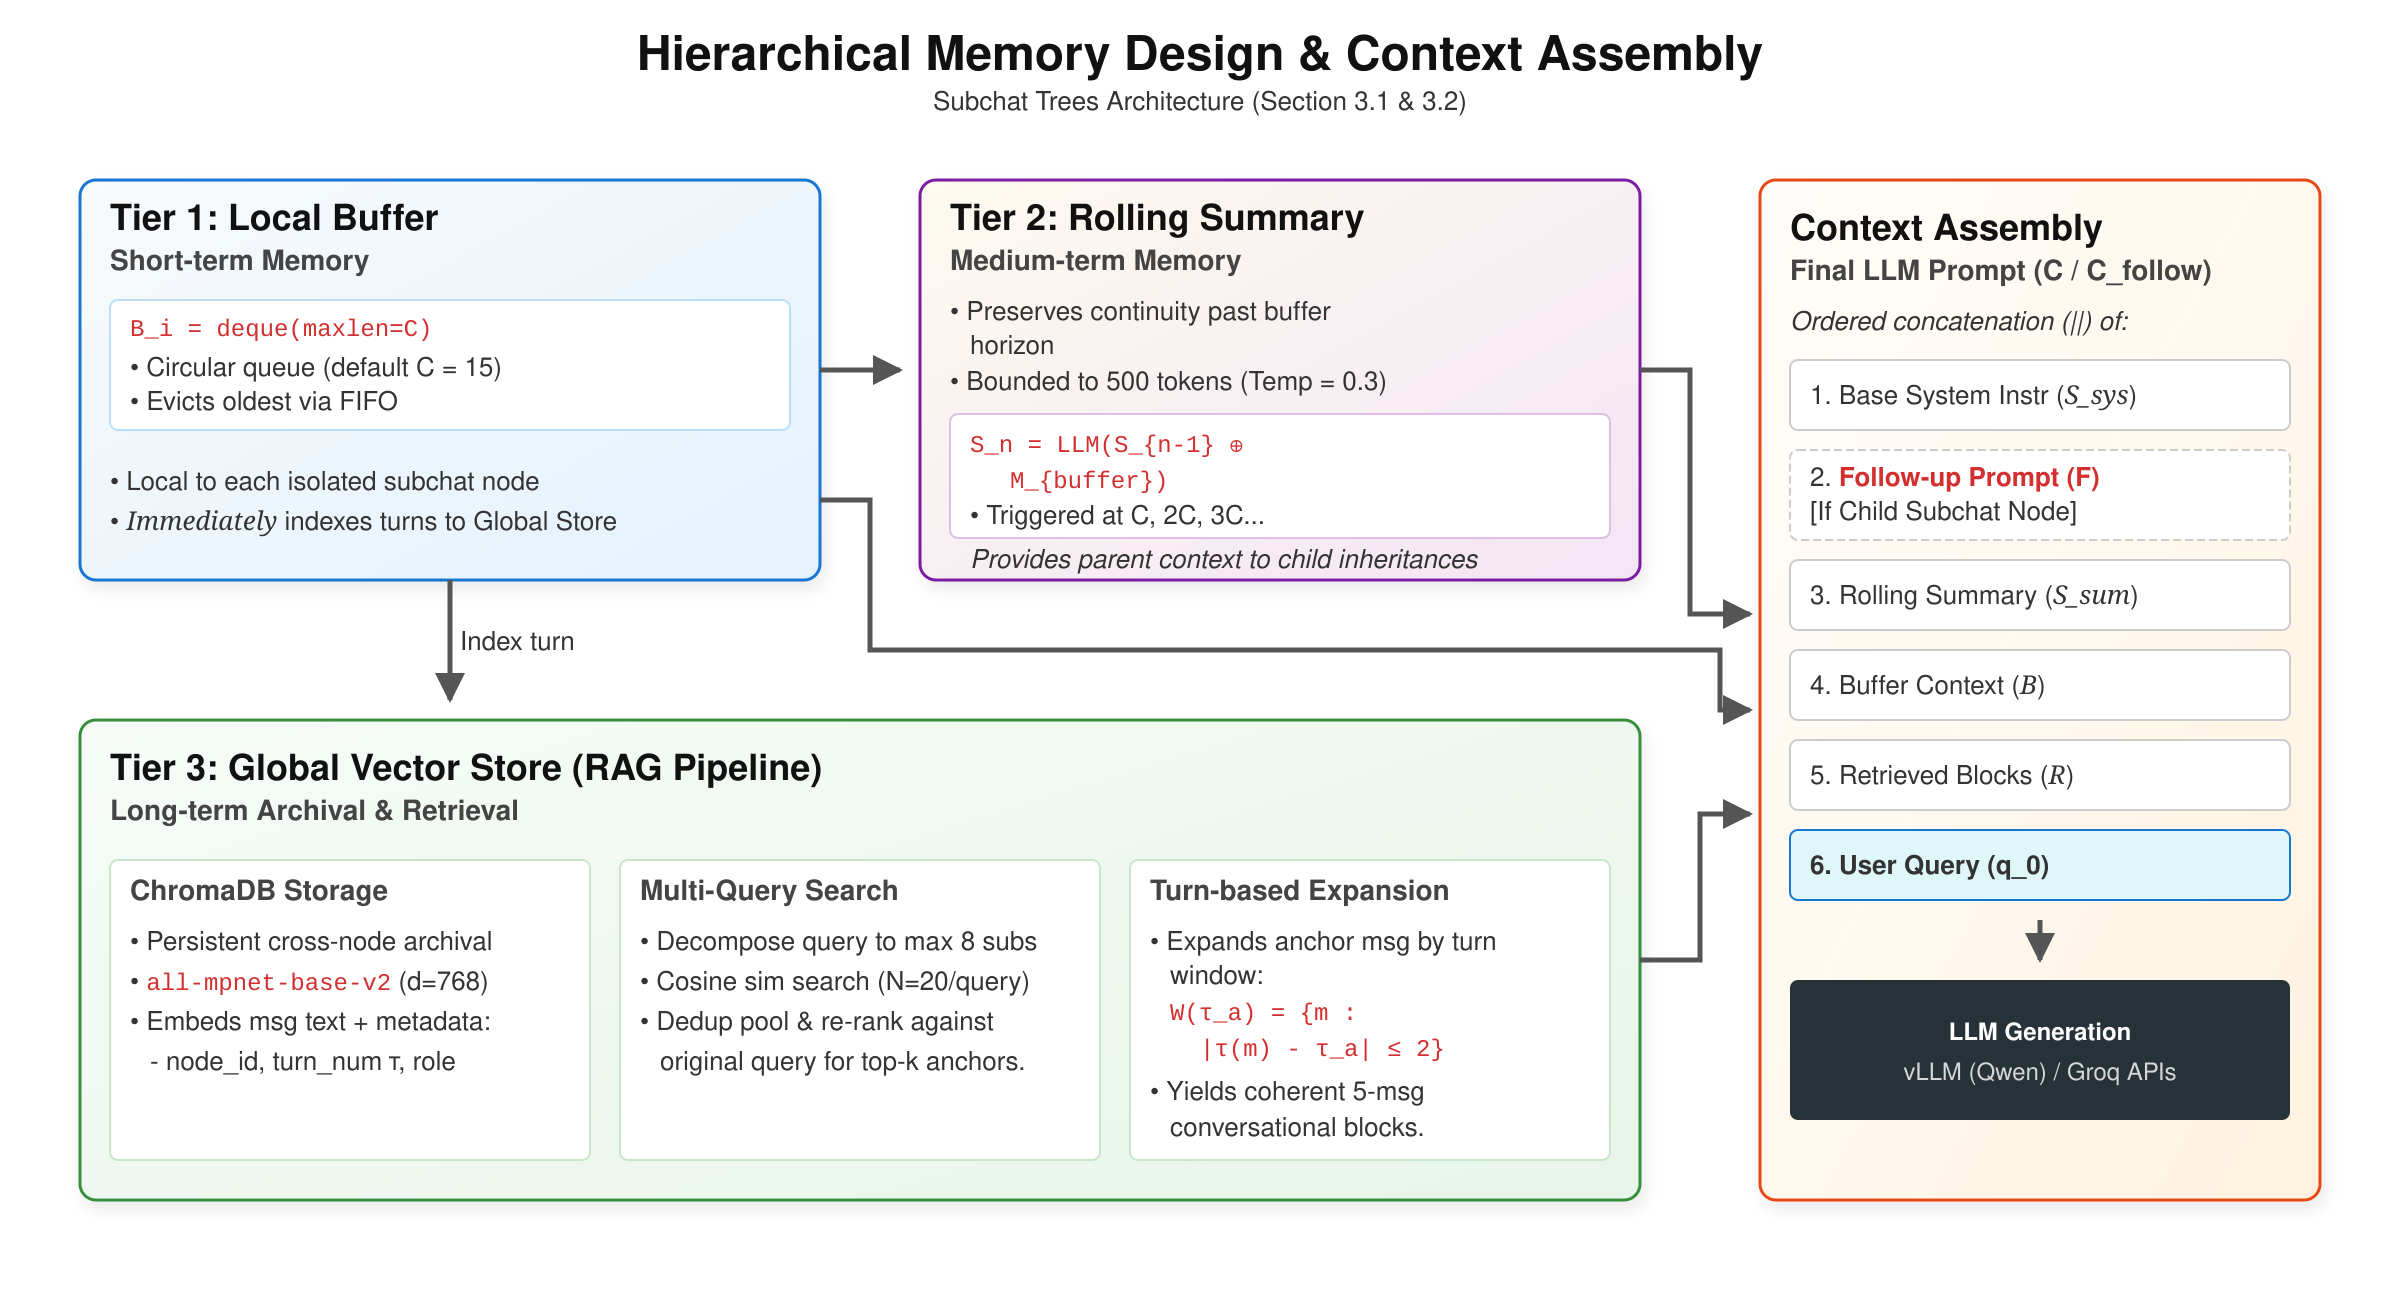
\includegraphics[width=0.90\paperheight,height=0.90\paperwidth,keepaspectratio]{diagrams/memory_design_academic.png}}};
\end{tikzpicture}
\null
\clearpage
\captionof{figure}{Three-tier memory design showing the relationship between the LocalBuffer (circular deque), rolling summarization, and vector store archival.}
\label{fig:memory}


\textbf{Tier~1: Local Buffer (Short-term Memory).}
Each node maintains a fixed-size circular buffer implemented as a \texttt{deque(maxlen=C)}:
\begin{equation}
B_i = \{(m_1, t_1), (m_2, t_2), \ldots, (m_C, t_C)\}
\label{eq:buffer}
\end{equation}
where $m_j$ is the $j$-th message, $t_j$ its timestamp, and $C$ the capacity. When $|B_i| > C$ or buffer limit reached, the oldest message is automatically evicted via FIFO policy. Crucially, messages are indexed to the global vector store \emph{immediately} upon addition (not upon eviction), ensuring up to date information availability during buffer turnover or node switching.

\textbf{Tier~2: Rolling Summarization (Medium-term Memory).}
To preserve semantic continuity beyond the buffer limit in long multi-turn conversation. A rolling summarization is triggered whenever the total message count reaches a multiple of the buffer size:
\begin{equation}
S_{n} = \text{LLM}_{\text{sum}}\!\left(S_{n-1} \oplus M_{\text{buffer}}\right), \quad \text{triggered at counts}\ C, 2C, 3C, \ldots
\label{eq:summary}
\end{equation}
where $S_n$ represent current summary, $S_{n-1}$ represent previous summary, $M_{\text{buffer}}$ is the complete set of messages currently in the buffer and $\oplus$ denotes concatenation. This dynamic triggering adapts to any buffer size without hard-coded thresholds. The summary is bounded at 500~tokens and generated at temperature $T{=}0.3$.

\textbf{Tier~3: Global Vector Store (Long-term Memory).}
All messages are embedded using \texttt{all-mpnet-base-v2} (SentenceTransformers, $d{=}768$) and stored in ChromaDB along with metadata:
\begin{equation}
\mathcal{V} = \left\{\left(\mathbf{e}(m),\; \text{meta}(m)\right) \;\middle|\; m \in \text{all messages}\right\}
\label{eq:vectorstore}
\end{equation}
where $\mathbf{e}(m) \in \mathbb{R}^{768}$ is the embedding and $\text{meta}(m)$ includes \texttt{node\_id}, \texttt{timestamp}, \texttt{role}, and \texttt{conversation\_title}. 

\subsection{Context Inheritance}\label{subsubsec:inheritance}

Creation of a child node $n_c$ from parent $n_p$:

\begin{equation}
\text{Context}(n_c) = \text{FollowUpPrompt}(n_c) \;\cup\; \text{BufferCopy}(n_p) \;\cup\; \text{SummaryInherit}(n_p)
\label{eq:inheritance}
\end{equation}

Specifically:
\begin{enumerate}
    \item \textbf{Buffer Inheritance:} All messages from the parent's buffer are copied into the child's buffer. This provides immediate conversational context.
    \item \textbf{Summary Inheritance:} The parent's rolling summary is also inherited. Transfering long term context to child.
    \item \textbf{Follow-up Prompt:} The selected text(parent's fragment) and user's intent (reason behind creating branch) are injected as a system message guiding the LLM's attention.
\end{enumerate}

The follow-up prompt is constructed as:
\begin{equation}
\text{FollowUpPrompt} = \texttt{``User selected:~''} \,\|\, s_{\text{sel}} \,\|\, \texttt{``~Focus on this.''}
\label{eq:followup}
\end{equation}

Here, subsequent messages in the child subchat do \emph{not} propagate back to the parent node, achieving bidirectional context isolation.

\subsection{Follow-up Mechanism}\label{subsubsec:followup_alg}

Algorithm~\ref{alg:subchat} formalizes the subchat creation process.

\begin{algorithm}[htbp]
\caption{Follow-up Subchat Creation}\label{alg:subchat}
\begin{algorithmic}[1]
\Require Parent node $n_p$, selected text $s_{\text{sel}}$, user query $q$, buffer size $C$
\Ensure Child node $n_c$ with isolated context
\State $n_c \gets \textsc{NewNode}(\text{parent}{=}n_p,\; C)$
\State $n_c.\text{context} \gets (s_{\text{sel}},\; \texttt{``follow\_up''})$
\State $\text{sys\_msg} \gets \textsc{BuildFollowUpPrompt}(s_{\text{sel}})$
\For{each message $m \in n_p.\text{buffer}$}
    \State $n_c.\text{buffer}.\textsc{Add}(m.\text{role},\; m.\text{text})$ \Comment{Inherit parent context}
\EndFor
\State $n_c.\text{summary} \gets n_p.\text{summary}$ \Comment{Inherit rolling summary}
\State $r \gets \text{LLM}\!\left(\text{sys\_msg} \;\|\; n_c.\text{buffer} \;\|\; q\right)$
\State $n_c.\text{buffer}.\textsc{Add}(\texttt{``user''},\; q)$
\State $n_c.\text{buffer}.\textsc{Add}(\texttt{``assistant''},\; r)$
\State \Return $n_c$
\end{algorithmic}
\end{algorithm}

\section{Vector Memory and RAG Pipeline}\label{subsec:rag}

The global vector store serves as long-term memory. It enables retrieval of relevant context from any point in any branch.

\subsection{Multi-Query Decomposition and Retrieval}\label{subsubsec:decomposition}

A single user query rarely captures all retrievable facets of a topic. Thus, the retrieval pipeline uses a four-phase process, 1. sub-query generation, 2. embedding-based vector search, 3. deduplication and 4. re-ranking. Figure~\ref{fig:retrieval_pipeline} illustrates the full flow.

\subsubsection{Sub-Query Generation.}
We prompt the LLM (Groq API, temperature~$T{=}0.3$) with intent-specific templates to decompose~$q$ into a set of sub-queries $Q = \{q_0, q_1, \dots, q_{n-1}\}$, where $q_0 = q$ is the original query and $q_1 \dots q_{n-1}$ are alternative query versions targeting related concepts, specific entities, or broader context ($n \leq 8$).






\subsubsection{Embedding and Vector Search.}
Each sub-query~$q_i$ is independently embedded using the \texttt{all-mpnet-base-v2} sentence-transformer model~\cite{reimers2019sentencebert}, producing a dense vector $e(q_i) \in \mathbb{R}^{768}$. Every indexed message in the system has been embedded with the same model and stored in a persistent ChromaDB~\cite{chromadb} collection. Each stored message also includes metadata fields such as \texttt{node\_id}, \texttt{role}, \texttt{timestamp}, \texttt{turn\_number}~$\tau$, \texttt{title}, and an \texttt{archived} flag. A cosine-similarity search retrieves top $N{=}20$ candidate messages per sub-query from the collection.

\subsubsection{Deduplication.}
Multiple sub-queries can return the same message. Thus, the system  deduplicate per sub-query (by content and message identifier), retaining at most $u = 5$ unique results each. A shared \emph{seen} set further removes cross-query duplicates. The candidate pool is then:
\begin{equation}
\mathcal{P} = \bigcup_{i=0}^{n-1} R_i, \quad |R_i| \leq u, \quad |\mathcal{P}| \leq n \cdot u
\label{eq:candidate_pool}
\end{equation}
where $R_i$ denotes the unique results for sub-query~$q_i$. A cosine-similarity re-ranking scores every candidate in~$\mathcal{P}$ against the original query~$q_0$ and returns the top-$k$ anchor messages ($k \in [3, 10]$, default~5) for downstream turn-based expansion (Section~\ref{subsubsec:window}).

\clearpage
\thispagestyle{empty}
\begin{tikzpicture}[remember picture,overlay]
\node at (current page.center) {
\includegraphics[width=0.90\paperwidth,height=0.90\paperheight,keepaspectratio]{diagrams/retrieval_pipeline.png}};
\end{tikzpicture}
\null
\clearpage
\captionof{figure}{End-to-end retrieval pipeline. \textbf{Phase~1}: LLM-based sub-query generation decomposes the user query into up to $n \leq 8$ sub-queries. \textbf{Phase~2}: each sub-query is embedded via \texttt{all-mpnet-base-v2} ($d{=}768$) and dispatched to ChromaDB for cosine search ($N{=}20$ candidates each), then deduplicated to $u{=}5$ unique results per sub-query. \textbf{Phase~3}: all anchor candidates are re-ranked by cosine similarity to the original query~$q_0$; top-$k$ are selected. \textbf{Phase~4}: each winning anchor expands $\pm\delta$ turns ($\delta{=}2$) into a coherent conversational block (Eq.~\ref{eq:window}). The resulting~$k$ blocks are injected into the LLM prompt.}
\label{fig:retrieval_pipeline}

\subsection{Context Window Retrieval}\label{subsubsec:window}

A retrieved message in isolation often lacks the conversational context necessary for coherent understanding. A na\"ive approach would define a temporal window (e.g.,\ $\pm 60$\,s around the anchor), but user response latencies are inconsistent and unpredictable---a reader may pause for seconds or minutes before replying---making time-based windows unreliable. We Therefore define a \emph{turn-based} context window anchored on conversational sequence.

Each message~$m$ is indexed with a monotonically increasing turn number $\tau(m)$ within its node. For an anchor message with turn number~$\tau_a$, the context window is:
\begin{equation}
W(\tau_a) = \left\{m \in M_{n} : |\tau(m) - \tau_a| \leq \delta\right\}
\label{eq:window}
\end{equation}
where $M_n$ is the set of all indexed messages in node~$n$ and $\delta = 2$ (i.e.,\ two turns before and two turns after the anchor). This yields at most $2\delta + 1 = 5$ messages per anchor regardless of the time elapsed between turns. As with temporal windows, we exclude any message still held in the active buffer:
\begin{equation}
W_{\mathrm{filtered}}(\tau_a) = W(\tau_a) \setminus B
\label{eq:window_filtered}
\end{equation}
here, $B$ denotes the current buffer contents.

Context expansion is applied \emph{after} re-ranking rather than before. The retrieval pipeline first re-ranks all deduplicated anchor candidates by cosine similarity to the original query~$q_0$ and selects the top-$k$ anchors ($k \in [3, 10]$, default~5). Only then does each winning anchor expand into its $\pm\delta$ turn window. This "\emph{rank-then-expand}" ordering ensures that neighbouring  messages never compete with anchors during ranking. Instead of that, each anchor is delivered to the LLM as a coherent conversational block rather than as scattered fragments interleaved with unrelated messages. Neighbour messages receive a discounted relevance score of $0.8 \times$ the anchor score. This helps preserving the distinction between directly matched content and its surrounding narrative.

\subsection{Context Assembly}\label{subsubsec:assembly}

The final prompt sent to the LLM is an ordered sequence of messages. Its composition differs depending on whether the active node is a \emph{root-level} conversation or a \emph{follow-up subchat}. Figure~\ref{fig:dataflow} illustrates both paths.

\clearpage
\thispagestyle{empty}
\begin{tikzpicture}[remember picture,overlay]
\node at (current page.center) {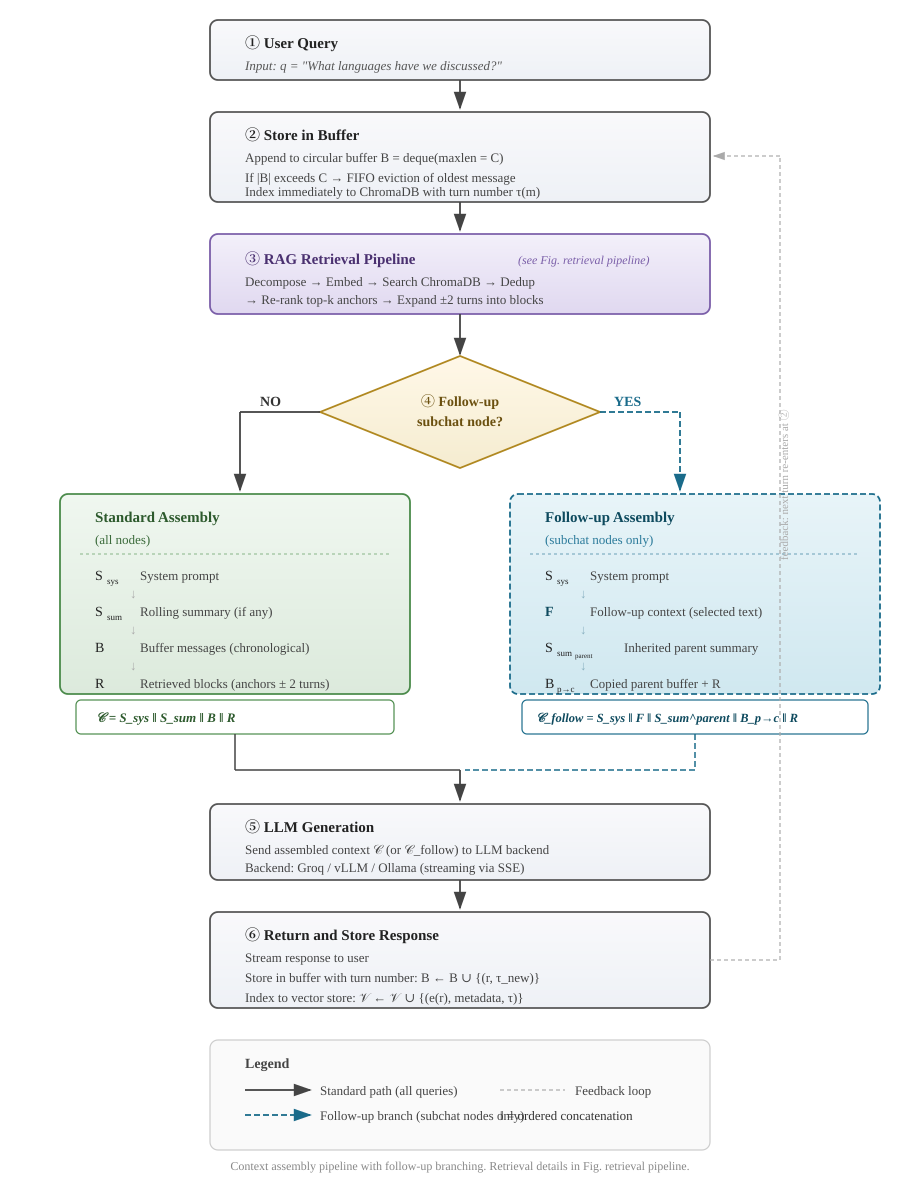
\includegraphics[width=0.90\paperwidth,height=0.90\paperheight,keepaspectratio]{diagrams/context_assembly_pipeline.png}};
\end{tikzpicture}
\null
\clearpage
\captionof{figure}{Context assembly pipeline. The user query is buffered (\textcircled{1}--\textcircled{2}) and passed through the RAG retrieval pipeline (\textcircled{3}; detailed in Figure~\ref{fig:retrieval_pipeline}), which returns coherent context blocks~$R$. At step~\textcircled{4} the pipeline branches: root-level nodes follow the \emph{standard} path (solid arrows, Eq.~\ref{eq:context_standard}), while follow-up subchat nodes additionally inject the selected-text prompt~$F$ and the inherited parent summary $S_{\mathrm{sum}}^{\,\mathrm{parent}}$ (dashed arrows, Eq.~\ref{eq:context_followup}). Both paths converge at step~\textcircled{5} for LLM generation, after which the response is stored back in the buffer and vector store (\textcircled{6}).}
\label{fig:dataflow}

\subsubsection{Standard Assembly (all nodes).}
Every query passes through the seven-step RAG pipeline described above. The assembled prompt takes the form:
\begin{equation}
\mathcal{C} = S_{\mathrm{sys}} \;\|\; S_{\mathrm{sum}} \;\|\; B \;\|\; R
\label{eq:context_standard}
\end{equation}
where $S_{\mathrm{sys}}$ is the base system instruction, $S_{\mathrm{sum}}$ is the node's rolling summary (omitted if none exists), $B$ is the circular buffer (recent turns in chronological order), $R$ is the set of retrieved messages returned by the RAG pipeline (empty when retrieval is not triggered), and $\|$ denotes ordered concatenation.

\subsubsection{Follow-up Assembly (subchat nodes).}
When a user selects text in a parent conversation and creates a subchat. The child node inherits three artifacts from its parent at creation time:
\begin{enumerate}
    \item \textbf{User intent prompt.} The text the user highlighted, along with users intent, is wrapped in a system message directing the model to focus on that specific topic.
    \item \textbf{Inherited summary.} The parent's rolling summary is copied to the child, providing long term context.
    \item \textbf{Parent buffer messages.} All messages currently in the parent's circular buffer are copied into the child's buffer. This ensures the child begins with the full recent context of the parent conversation.
\end{enumerate}
The resulting prompt becomes:
\begin{equation}
\mathcal{C}_{\mathrm{follow}} = S_{\mathrm{sys}} \;\|\; F \;\|\; S_{\mathrm{sum}}^{\,\mathrm{parent}} \;\|\; B_{\mathrm{parent} \to \mathrm{child}} \;\|\; R
\label{eq:context_followup}
\end{equation}
where $F$ is the follow-up context, $S_{\mathrm{sum}}^{\,\mathrm{parent}}$ is the inherited parent summary, and $B_{\mathrm{parent} \to \mathrm{child}}$ denotes the child's buffer initialized with the parent's messages. As the child conversation progresses, new turns are appended to this buffer (evicting older ones via FIFO), and its own rolling summary gradually replaces the inherited one, ensuring continuity while allowing topic divergence. But parent's state remain unchanged.

\section{User Interface}\label{subsec:ui}

\subsection{Design Rationale.}
The interface deliberately adopts a messenger-style layout---a familiar paradigm shared by WhatsApp, iMessage, and Slack---so that users can transfer existing mental models to the new system without additional learning overhead~\cite{nielsen1994usability}. By anchoring interaction in a well-understood pattern (send a message, receive a reply), the cognitive cost of the novel \emph{subchat} mechanism is kept low.

\subsection{The Problem with Linear Chat.}
Conventional LLM chat interfaces present all exchanges in a single, chronologically ordered thread. As conversations grow in length or branch across topics, this layout introduces several usability failures: (i)~users must scroll extensively to relocate earlier context, (ii)~there is no affordance for branching---returning to a prior topic forces the user to re-state context or risk contaminating the current thread, and (iii)~the model's fixed context window silently evicts earlier turns, creating an invisible boundary between what the user remembers and what the model can still ``see.'' These issues compound in exploratory or multi-topic sessions.

\subsection{Subchat Trees as a Solution.}
Our interface exposes the underlying tree structure through two complementary views (Figure~\ref{fig:ui}): a collapsible \emph{tree navigator} on the left and a focused \emph{chat panel} on the right. Users create a subchat by selecting any text in the chat panel and clicking a single button; the new subchat inherits relevant context (Section~\ref{subsubsec:assembly}) without disrupting the parent conversation. This design follows the principle of \emph{progressive disclosure}~\cite{norman2013design}: the default view is a simple chat, but richer structure (branching, parallel follow-ups, hierarchical navigation) is available on demand.

\clearpage
\thispagestyle{empty}
\begin{tikzpicture}[remember picture,overlay]
\node at (current page.center) {\rotatebox{90}{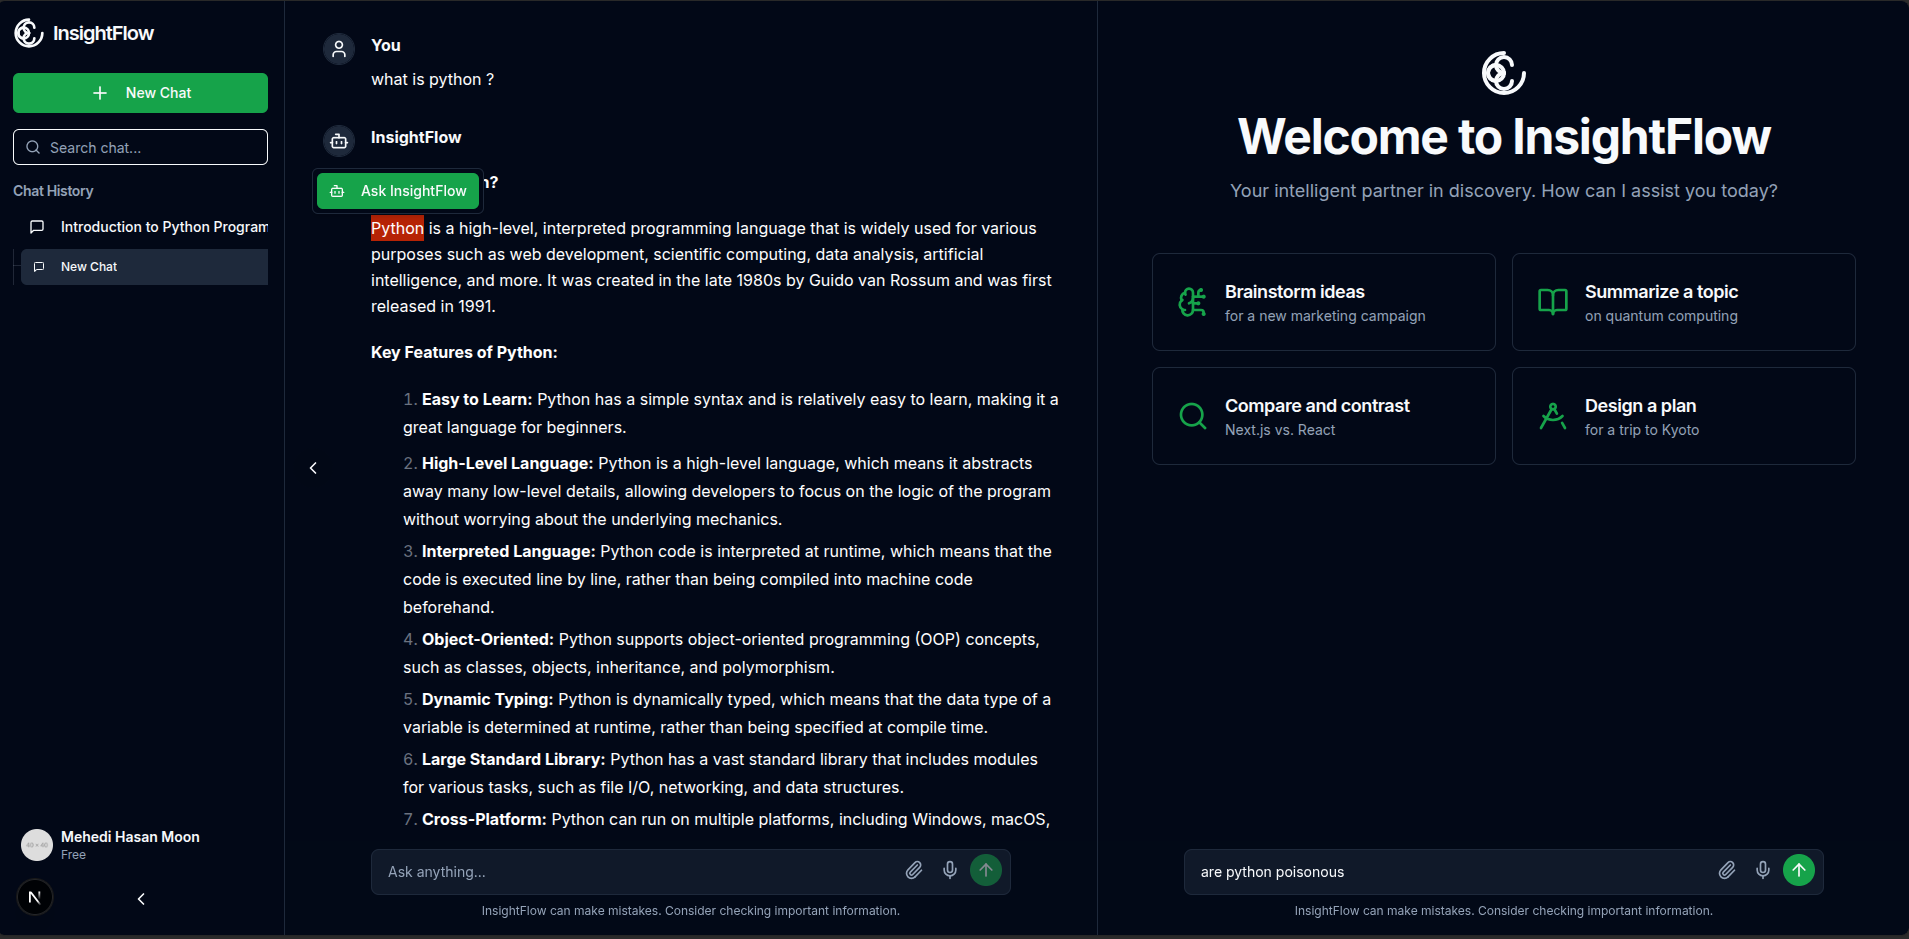
\includegraphics[width=0.90\paperheight,height=0.90\paperwidth,keepaspectratio]{diagrams/frontend.png}}};
\end{tikzpicture}
\null
\clearpage
\captionof{figure}{User interface: (left) the conversation forest tree view with expandable nodes, and (right) the chat panel with text selection for one-click subchat creation.}
\label{fig:ui}

Key affordances include: (i)~breadcrumb navigation showing the path from root to the active subchat, (ii)~visual indicators for inherited context and active retrieval status, (iii)~parallel follow-ups that let users explore multiple branches of a topic simultaneously, and (iv)~real-time token streaming via Server-Sent Events across multiple LLM backends (Groq, vLLM, Ollama).

\section{Baseline System}\label{subsec:baseline}

For comparison, we implement a linear chat baseline:
\begin{itemize}
    \item Single conversation thread with a shared circular buffer ($C$ messages, FIFO eviction).
    \item All topics share the same context window---no isolation mechanism.
    \item Identical LLM backend, embedding model, and temperature settings.
\end{itemize}
Both systems use the same buffer capacity $C$ in each experiment, isolating the effect of conversation structure.

\section{System Development}
% \subsection{Technology Stack}\label{subsubsec:stack}

% \begin{itemize}
%     \item \textbf{Backend:} FastAPI (Python~3.12), stateless design for horizontal scaling.
%     \item \textbf{LLM (Cloud):} Groq API support for hosted inference and tool-calling configurations.
%     \item \textbf{LLM (Local GPU):} vLLM with Qwen-2.5 14B Instruct AWQ~\cite{qwen2025qwen25} (4-bit quantization) on Kaggle T4 GPUs.
%     \item \textbf{Vector DB:} ChromaDB with \texttt{all-mpnet-base-v2} embeddings ($d{=}768$).
%     \item \textbf{Frontend:} Next.js~14, TypeScript, with Server-Sent Events for streaming.
%     \item \textbf{Testing:} Custom Python harness with deterministic topic-prefix scoring and ChromaDB clearing between runs.
% \end{itemize}

\begin{table}[htbp]
\caption{LLM temperature settings by task.}\label{tab:temps}
\begin{tabular*}{\textwidth}{@{\extracolsep\fill}lcc@{}}
\toprule
\textbf{Task} & \textbf{Temperature} & \textbf{Rationale} \\
\midrule
Main conversation  & 0.3 & Deterministic replay \\
Title generation   & 0.3 & Consistent naming \\
Summarization      & 0.3 & Structured output \\
Topic-prefix scoring & --- & Deterministic regex evaluation \\
Query decomposition & 0.3 & Structured retrieval \\
\botrule
\end{tabular*}
\end{table}

% \subsection{Serverless Kaggle Evaluation Harness}\label{subsubsec:kaggle}

% A key design choice is our \emph{serverless} evaluation harness, which enables fully reproducible experiments from a single Kaggle notebook. The traditional evaluation path routes requests through a FastAPI HTTP server; however, on GPU-constrained cloud notebooks, maintaining a separate server process alongside the vLLM model is impractical.

% Our serverless runner eliminates this overhead by directly importing and instantiating the core backend classes (\texttt{SimpleChat}, \texttt{ChatGraphManager}, \texttt{Forest}, \texttt{TreeNode}, and the vector-memory components) within the same Python process as the vLLM model. The workflow proceeds as follows:

% \begin{enumerate}
%     \item \textbf{Model Loading:} vLLM loads Qwen-2.5 14B Instruct AWQ with 4-bit quantization, utilizing 91\% of available GPU memory (\texttt{gpu\_memory\_utilization=0.91}), with \texttt{max\_model\_len=5000} and prefix caching enabled.
%     \item \textbf{Registration:} The loaded model is registered globally via \texttt{VLLMClient.set\_model(llm)}, making it available to all backend components for response generation and rolling summarization without network hops.
%     \item \textbf{Inference:} Prompts are formatted using the Hugging Face tokenizer's native \texttt{apply\_chat\_template()}, ensuring correct special tokens for the Qwen chat format. Single-batch offline inference via \texttt{llm.generate()} avoids HTTP serialization overhead.
%     \item \textbf{State Management:} Between baseline and system tests, all node maps and forest state are cleared, and the vector index collection is reset to prevent cross-condition leakage.
%     \item \textbf{Logging:} After each buffer size completes, the runner writes Markdown tables, raw JSON metrics, recall-probe outputs, and component logs to the buffer-specific results directory.
% \end{enumerate}

% This architecture ensures that response generation and rolling summarization use the same in-process model, while topic-prefix scoring remains deterministic and independent of any judge model.

% 
